\chapter{Lange Strings und die Schwarze-Loch-Korrespondenz}

\lectureoverview{Ein Schwarzes Loch besitzt eine Entropie und muss daher mikroskopische Freiheitsgrade haben. Wir entwickeln die einfachste stringtheoretische Beschreibung dieser Freiheitsgrade: Zuerst zählen wir die Zustände einer langen angeregten Saite, dann variieren wir die Stringkopplung, bis die Beschreibungen durch String und Schwarzes Loch ineinander übergehen. Die abschließende Gleichheit bleibt bewusst als Aufgabe für die nächste Vorlesung offen.}

\section{Entropie setzt mikroskopische Träger voraus}

Wenn wir sagen, ein System habe eine große Entropie, meinen wir, dass es eine große Menge mikroskopischer Information verbergen kann. Eine Badewanne voll heißem Wasser kann eine Entropie in der Größenordnung von \(10^{30}\) haben. Diese Aussage allein verrät uns bereits, dass es enorm viele mikroskopische Freiheitsgrade gibt – unabhängig davon, ob wir sie Molekül für Molekül untersuchen. Die Thermodynamik kann die Entropie durch Messung von Energie und Temperatur bestimmen, identifiziert aber nicht die Objekte, die sie tragen.

Die Unterscheidung ist aus der Strömungsmechanik vertraut. Sie beschreibt Dichte, Geschwindigkeit, Druck und makroskopische Strömung, ohne auf Atome Bezug zu nehmen. Ergänzt man die Thermodynamik, zeigt sich, dass eine Flüssigkeit Entropie besitzt. Die Entropie weist auf eine mikroskopische Struktur hin, die in den gemittelten Gleichungen nicht sichtbar ist; sie wirft eine neue Frage auf, statt sie zu beantworten.

Schwarze Löcher stellen dieselbe Herausforderung in zugespitzter Form. Bekensteins Vorschlag, den Hawkings Berechnung vervollständigte, ordnet ihnen eine zur Horizontfläche proportionale Entropie zu. Die allgemeine Relativitätstheorie bestimmt die Geometrie und ihre Thermodynamik, liefert aber keine Aufstellung der mikroskopischen Zustände. Was sind die kleinen, zahlreichen Objekte, deren Konfigurationen das Flächengesetz erklären? In der Stringtheorie gibt es einen konkreten Kandidaten. Die hier entwickelte Argumentation ist bewusst qualitativ: Sie ergibt die richtige parametrische Abhängigkeit, lässt aber numerische Konstanten und den formalen Apparat einer vollständigen Zustandszählung außer Acht.

\section{Drei Skalen und eine tückische Notation}

Die Gravitation zeichnet eine charakteristische Länge aus, die Planck-Länge,
\begin{equation}
\ell_p=\sqrt{\frac{G_N\hbar}{c^3}}.
\label{eq:l06-planck-si}
\end{equation}

\begin{classroomqa}\audiencequestion{Welche Kombination aus \(G_N\), \(\hbar\) und \(c\) ergibt die Planck-Länge?\lecturetimestamp{00:06:08}}\lecturerresponse{Es ist \(\sqrt{G_N\hbar/c^3}\), also etwa \(10^{-33}\) Zentimeter. Wir setzen sofort \(\hbar=c=1\); damit wird der Zusammenhang viel einfacher.}\end{classroomqa}

In natürlichen Einheiten gilt
\begin{equation}
\hbar=c=1,
\qquad
G_N=\ell_p^2.
\label{eq:l06-planck-area}
\end{equation}
Damit hat die Newton-Konstante die Dimension einer Fläche. Deshalb ist eine Fläche dividiert durch \(G_N\) dimensionslos und kann als Entropie auftreten.

Die Stringtheorie besitzt eine zweite Länge, \(\ell_s\). Erhitzt man eine Saite oder versetzt sie in einen hoch angeregten Zustand, schwingt sie auf vielen Skalen. In diesem einfachen Bild ist die charakteristische kürzeste Skala die Stringlänge. Man kann \(\ell_s\) als die Größe auffassen, die einer elementaren Schwingungseinheit der Saite entspricht.

Die dritte Größe ist die dimensionslose Stringkopplung \(g_s\). Sie steuert Aufspaltung und Vereinigung: Eine Saite kann sich in zwei Saiten aufspalten, oder eine angeregte Saite kann ein Quant des geschlossenen Strings emittieren.

\begin{classroomqa}\audiencequestion{Welche physikalische Bedeutung hat die Stringkopplung?\lecturetimestamp{00:09:20}}\lecturerresponse{Sie bestimmt die Wahrscheinlichkeit einer Stringwechselwirkung, etwa einer Aufspaltung, wenn eine Saite sich selbst kreuzt. Genauer gesagt ist \(g_s\) die Wechselwirkungsamplitude; eine entsprechende Wahrscheinlichkeit oder Rate beginnt in der Ordnung \(g_s^2\).}\end{classroomqa}

Die emittierte masselose Anregung des geschlossenen Strings kann ein Graviton sein. In dieser Hinsicht spielt \(g_s\) eine ähnliche Rolle wie die elektrische Ladung: Sie ist der Faktor, der an einem Wechselwirkungsscheitelpunkt auftritt.\editorialnote{In der Vorlesung wird \(g_s\) abwechselnd als Wahrscheinlichkeit und als Amplitude bezeichnet. In der Störungstheorie ist sie die Kopplung auf Amplitudenebene; Wahrscheinlichkeiten und Raten enthalten ihr Quadrat.}

\section{Warum die Gravitation etwas über \texorpdfstring{\(g_s^2\)}{die Kopplung im Quadrat}}

Betrachten wir zunächst das Austauschbild der Elektromagnetik. Ein geladenes Objekt emittiert ein Photon mit einem Faktor \(e\), ein zweites absorbiert es mit einem weiteren Faktor \(e\). Die Austauschamplitude enthält daher \(e^2\). Das Bild beschreibt keine wörtliche klassische Geschichte mit einem Teilchen als Geschoss, zeigt aber zutreffend, wie die Kopplung eingeht.

\begin{figure}[htbp]\centering
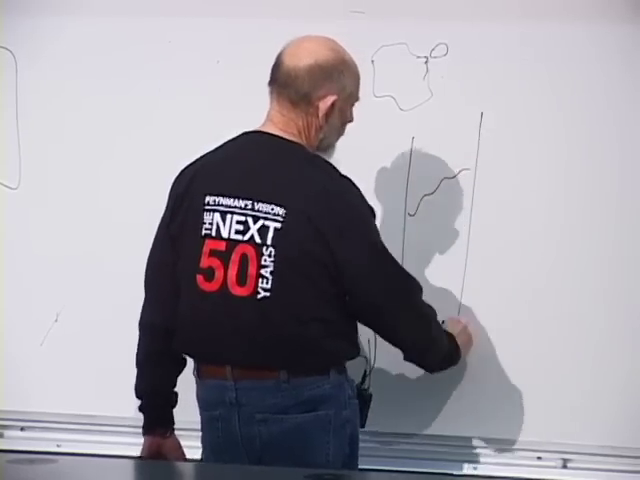
\includegraphics[width=0.72\textwidth]{lecture_06_figure_03.png}\caption{Die vervollständigten Austauschschaubilder an der Tafel: Bei der Emission tritt ein Kopplungsfaktor auf und bei der Absorption erneut.}\lectureframe{00:11:30.000}\end{figure}

In der Stringtheorie wird das Photon durch ein Graviton und die elektrische Ladung durch \(g_s\) ersetzt. Ein Faktor gehört zur Emission, ein weiterer zur Absorption, sodass die Stärke der Gravitation mit \(g_s^2\) skaliert.

Bei großen Abständen muss dieselbe Wechselwirkung das Newtonsche Kraftgesetz reproduzieren,
\begin{equation}
F_{\mathrm{grav}}\sim G_N\frac{M_1M_2}{r^2}.
\end{equation}
Die Massen und die Abhängigkeit vom inversen Quadrat beschreiben die Quellen und die Ausbreitung; hier kommt es auf die Kopplung an, die sie multipliziert.

\begin{figure}[htbp]\centering
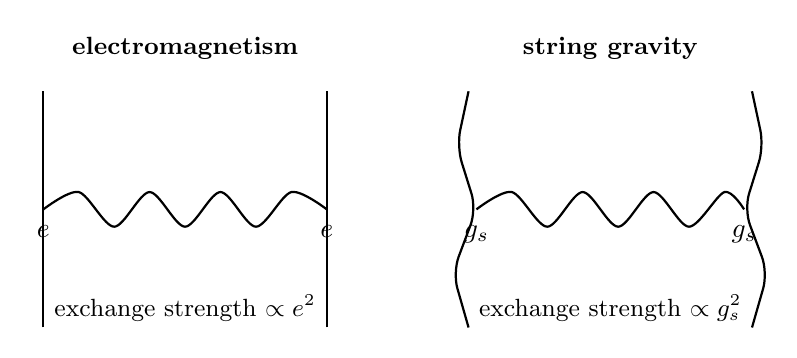
\begin{tikzpicture}[x=1cm,y=1cm]
  \node[font=\small\bfseries] at (1.8,3.55) {electromagnetism};
  \draw[line width=0.8pt] (0,0) -- (0,3);
  \draw[line width=0.8pt] (3.6,0) -- (3.6,3);
  \draw[line width=0.8pt] plot[smooth] coordinates {(0,1.5) (0.45,1.72) (0.9,1.28) (1.35,1.72) (1.8,1.28) (2.25,1.72) (2.7,1.28) (3.15,1.72) (3.6,1.5)};
  \node[below] at (0,1.42) {\(e\)};
  \node[below] at (3.6,1.42) {\(e\)};
  \node[font=\small] at (1.8,0.25) {exchange strength \(\propto e^2\)};
  \node[font=\small\bfseries] at (7.2,3.55) {string gravity};
  \draw[line width=0.8pt,rounded corners=6pt] (5.4,0) -- (5.2,0.7) -- (5.5,1.5) -- (5.25,2.3) -- (5.4,3);
  \draw[line width=0.8pt,rounded corners=6pt] (9,0) -- (9.2,0.7) -- (8.9,1.5) -- (9.15,2.3) -- (9,3);
  \draw[line width=0.8pt] plot[smooth] coordinates {(5.5,1.5) (5.95,1.72) (6.4,1.28) (6.85,1.72) (7.3,1.28) (7.75,1.72) (8.2,1.28) (8.65,1.72) (8.9,1.5)};
  \node[below] at (5.5,1.42) {\(g_s\)};
  \node[below] at (8.9,1.42) {\(g_s\)};
  \node[font=\small] at (7.2,0.25) {exchange strength \(\propto g_s^2\)};
\end{tikzpicture}\caption{Die Analogie beim Abzählen der Kopplungsfaktoren. Jedes Ende des ausgetauschten Quants trägt einen Wechselwirkungsfaktor bei.}\end{figure}

Diese Beobachtung legt die Newton-Konstante beinahe fest. Die Kopplung \(g_s\) ist dimensionslos, während \(G_N\) in vier Dimensionen die Dimension einer Länge zum Quadrat hat. Die verfügbare mikroskopische Länge ist \(\ell_s\), also gilt
\begin{equation}
G_N\sim g_s^2\ell_s^2.
\label{eq:l06-newton-string}
\end{equation}
Zusammen mit Gleichung~\eqref{eq:l06-planck-area} folgt
\begin{equation}
\ell_p\sim g_s\ell_s.
\label{eq:l06-planck-string}
\end{equation}

\begin{figure}[htbp]\centering
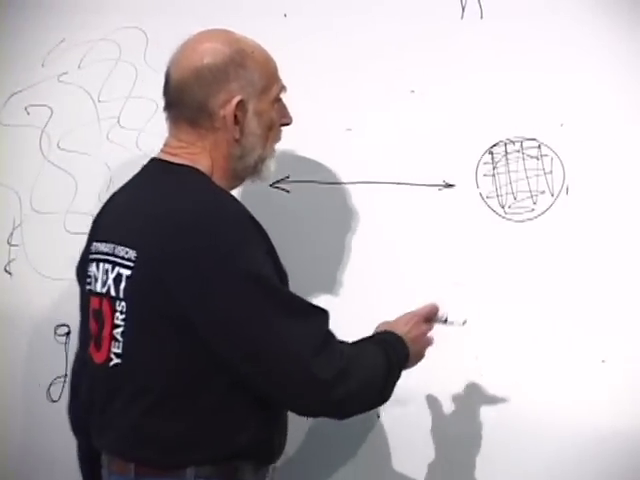
\includegraphics[width=0.72\textwidth]{lecture_06_figure_04.png}\caption{Die grundlegenden Beziehungen an der Tafel: \(\ell_p^2=G_N\) und \(\ell_p\sim g_s\ell_s\).}\lectureframe{00:15:45.000}\end{figure}

Gleichung~\eqref{eq:l06-newton-string} ist der vereinfachte Zusammenhang, den wir in dieser Vorlesung durchgehend verwenden.\editorialnote{In einer kompaktifizierten Stringtheorie hängt die effektive vierdimensionale Newton-Konstante auch vom Kompaktifizierungsvolumen und von Konventionen mit Faktoren der Größenordnung eins ab. Die Vorlesung lässt diese Größen außer Acht, um die Skalierung der Korrespondenz herauszuarbeiten.}

\begin{classroomqa}\audiencequestion{Ist \(g_s\) größer oder kleiner als eins, und welche Länge ist größer?\lecturetimestamp{00:16:00}}\lecturerresponse{Wir arbeiten bei schwacher Kopplung, \(g_s<1\). Dann bedeutet \(\ell_p\sim g_s\ell_s\), dass die Stringlänge größer als die Planck-Länge ist. Starke Kopplung erfordert eine andere Beschreibung, die wir hier nicht benötigen.}\end{classroomqa}

\section{Die Zählung für Schwarze Löcher}

Unter Weglassung der Boltzmann-Konstante und numerischer Faktoren lautet die Bekenstein--Hawking-Entropie
\begin{equation}
S_{\mathrm{BH}}=\frac{A}{4G_N}sim\frac{A}{G_N}sim\frac{A}{\ell_p^2}.
\label{eq:l06-bh-area}
\end{equation}
Der Faktor \(1/4\) ist in der semiklassischen Formel exakt, spielt für dieses Skalierungsargument aber keine Rolle.

\begin{classroomqa}\audiencequestion{Steht der Index ``BH'' für Schwarzes Loch oder für Bekenstein--Hawking?\lecturetimestamp{00:16:51}}\lecturerresponse{Für unsere Zwecke kann er an beides erinnern. Entscheidend ist die Aussage, dass die Entropie der Horizontfläche, gemessen in Planck-Flächen, entspricht.}\end{classroomqa}

Für ein vierdimensionales Schwarzschild-Schwarzes-Loch gilt
\begin{equation}
R_s=2G_NM,
\qquad
A=4\pi R_s^2.
\end{equation}
Lassen wir, wie in der Vorlesung, \(2\) und \(4\pi\) weg,
\begin{align}
S_{\mathrm{BH}}
&\sim \frac{R_s^2}{G_N}
\sim \frac{(G_NM)^2}{G_N} \\
&\sim M^2G_N
\sim M^2\ell_p^2.
\label{eq:l06-bh-mass}
\end{align}
Dies ist die Form, die wir mit einer Stringzählung vergleichen werden.

\section{Eine lange Saite als Zufallsweg}

Wir beginnen mit einer kurzen Saite und führen ihr Energie zu. Eine typische hoch angeregte Saite bleibt keine ordentliche Schleife. Sie wird zu einem langen, verwickelten Objekt – wie eine Angelschnur, die sich auf einer verhedderten Rolle verknotet hat. Dieses Knäuel besitzt Entropie, weil es enorm viele Konfigurationen gibt, die makroskopisch gleich aussehen.

Um sie zu zählen, ersetzen wir den Raum durch ein Gitter mit Kanten der Länge \(\ell_s\). Die Ecken sind die Gitterpunkte, die Kanten die Linien und die elementaren Quadrate die Flächen. Eine Saite wird als zusammenhängende Folge von Kanten dargestellt. Dieses Modell ist bewusst grob, doch seine exponentielle Zustandszahl erfasst die gesuchte Skalierung.

\begin{figure}[htbp]\centering
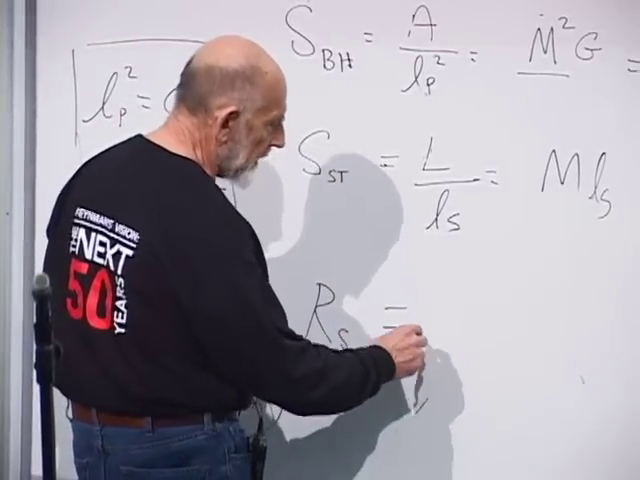
\includegraphics[width=0.72\textwidth]{lecture_06_figure_05.png}\caption{Das zweidimensionale Gittermodell. Das blaue Segment markiert einen Schritt der Saite; an jedem Gitterpunkt werden die vier möglichen Fortsetzungen gezählt.}\lectureframe{00:23:50.000}\end{figure}

\begin{classroomqa}\audiencequestion{Wie viele Wahlmöglichkeiten gibt es bei jedem Schritt des Modellwegs?\lecturetimestamp{00:22:43}}\lecturerresponse{Auf dem quadratischen Gitter sind es vier, da unmittelbares Zurückgehen erlaubt ist. In drei Dimensionen wären es sechs. Bei einem anderen Gitter ändert sich die konkrete Zahl, nicht aber die Tatsache, dass die Zahl der Wege exponentiell mit der Anzahl der Kanten wächst.}\end{classroomqa}

Hat die Saite \(n\) Kanten, so ergibt sich für das zweidimensionale Modell die Zählung
\begin{equation}
\Omega_n\sim4^n.
\label{eq:l06-walk-count}
\end{equation}
Es gibt einen einzigen Ausnahmefall, den geradlinigen Weg, aber das ist nur ein Zustand unter \(4^n\). Ein typischer Weg faltet sich wiederholt und füllt ein verwickeltes Knäuel aus. Für große \(n\) sieht fast jede zufällig erzeugte Konfiguration qualitativ wie jede andere aus.

Die Entropie ist der Logarithmus der Anzahl makroskopisch ununterscheidbarer Konfigurationen:
\begin{equation}
S_{\mathrm{st}}=\log\Omega_n\sim n\log4\sim n.
\label{eq:l06-string-entropy-n}
\end{equation}

\begin{classroomqa}\audiencequestion{Warum ist die Entropie proportional zu \(n\) und nicht zu \(4^n\)?\lecturetimestamp{00:25:39}}\lecturerresponse{Die Entropie ist der Logarithmus der Zustandszahl. Also gilt \(\log(4^n)=n\log4\); den Faktor \(\log4\), eine Konstante der Größenordnung eins, lassen wir weg.}\end{classroomqa}

Ist \(L\) die Länge entlang der Saite, gemessen von einem Ende bis zum anderen, so gilt
\begin{equation}
n=\frac{L}{\ell_s},
\qquad
S_{\mathrm{st}}\sim\frac{L}{\ell_s}.
\label{eq:l06-string-entropy-length}
\end{equation}
Hier ist \(L\) nicht der Durchmesser des verwickelten Knäuels. Gemeint ist die viel größere Strecke entlang der Saite.

Als Nächstes ersetzen wir die Länge entlang der Saite durch die Masse. Bei \(c=\hbar=1\) hat die Masse die Dimension einer inversen Länge. Eine Kante von der Größe einer Stringlänge trägt daher eine Masse der Größenordnung
\begin{equation}
m_{\mathrm{link}}\sim\frac{1}{\ell_s}.
\label{eq:l06-link-mass}
\end{equation}

\begin{classroomqa}\audiencequestion{Warum muss die Masse einer Kante mit \(1/\ell_s\) skalieren?\lecturetimestamp{00:29:20}}\lecturerresponse{In diesen Einheiten ist die Masse eine inverse Länge, und \(\ell_s\) ist die einzige verfügbare Länge. Äquivalent dazu ergibt eine Stringspannung der Größenordnung \(1/\ell_s^2\) multipliziert mit einer Kantenlänge \(\ell_s\) dasselbe Resultat.}\end{classroomqa}

Für die gesamte Saite gilt dann
\begin{equation}
M\sim n m_{\mathrm{link}}
\sim\frac{n}{\ell_s}
\sim\frac{L}{\ell_s^2},
\qquad
L\sim M\ell_s^2.
\label{eq:l06-string-mass}
\end{equation}
Einsetzen in Gleichung~\eqref{eq:l06-string-entropy-length} ergibt
\begin{equation}
S_{\mathrm{st}}\sim M\ell_s.
\label{eq:l06-string-entropy-mass}
\end{equation}
Der Gitterweg berücksichtigt weder die Zwangsbedingungen auf dem Weltblatt noch numerische Koeffizienten. Das exponentielle Wachstum des Spektrums hoch angeregter Saiten liefert jedoch dieselbe führende Skalierung.\editorialnote{Die Zufallsweg-Konstruktion dient als Merkhilfe für die Zustandsdichte der Saite bei hohen Anregungen; sie ist keine wörtliche Diskretisierung einer fundamentalen Saite.}

\section{Die Diskrepanz, die das Argument in Gang setzt}

Die beiden Ergebnisse lauten nun
\begin{equation}
S_{\mathrm{BH}}\sim M^2\ell_p^2,
\qquad
S_{\mathrm{st}}\sim M\ell_s.
\label{eq:l06-two-entropies}
\end{equation}
Sie ähneln einander, sind aber bei fester Masse und beliebiger Kopplung nicht gleich. Der Ausdruck für das Schwarze Loch ist quadratisch in \(M\), der für die Saite linear. Wir können eine heiße Saite nicht einfach zum Schwarzen Loch erklären, ohne zu erläutern, wie die beiden Bereiche ineinander übergehen.

\begin{figure}[htbp]\centering
\includegraphics[width=0.78\textwidth]{lecture_06_figure_06.png}\caption{Der ungehinderte Vergleich an der Tafel: oben die Entropie des Schwarzen Lochs, unten die der langen Saite; links die Beziehungen zwischen Planck- und Stringlänge.--}\lectureframe{00:33:20.000}\end{figure}

Hier legte die Vorlesung eine Pause ein. Die Spannung ist nützlich: Die Diskrepanz widerlegt die Idee nicht, sondern ist der Hinweis darauf, dass wir denselben Zustand vergleichen müssen, während wir die Stärke der Gravitation verändern.

\section{Den Kopplungsregler drehen}

Wir halten \(\ell_s\) fest und stellen uns vor, \(g_s\) lasse sich verändern. Bei \(g_s=0\) spalten sich Strings weder auf noch vereinigen sie sich, und die Gravitation verschwindet, weil \(G_N\sim g_s^2\ell_s^2\). Ein hinreichend energiereicher Zustand ist dann eine lange, schwach wechselwirkende Saite.

Wir erhöhen \(g_s\) langsam. Stringwechselwirkungen werden möglich, und – wichtiger für das gegenwärtige Argument – die Gravitation wird stärker.

\begin{classroomqa}\audiencequestion{Ist der erste Effekt einer Zunahme von \(g_s\) einfach, dass sich die Saite in kürzere Saiten aufspaltet?\lecturetimestamp{00:36:29}}\lecturerresponse{Aufspaltungen und Vereinigungen werden möglich. Wir halten aber \(\ell_s\) fest und verfolgen den Zustand hoher Entropie. Entscheidend ist, dass \(G_N\) wächst und damit die Eigengravitation der langen Saite das verwickelte Knäuel zusammenzieht.}\end{classroomqa}

Das Objekt zieht sich zusammen und wird dichter. Seine gravitative potenzielle Energie ist negativ; durch die Kontraktion sinkt daher seine Gesamtenergie und folglich seine Masse.

\begin{classroomqa}\audiencequestion{Nimmt die Energie zu oder ab, wenn die Eigengravitation die Saite zusammenzieht?\lecturetimestamp{00:37:48}}\lecturerresponse{Sie nimmt ab. Die Bindungsenergie wird negativer. Die Masse entlang dieses Verlaufs muss nicht konstant bleiben, auch wenn wir weiterhin denselben Zustand verfolgen.}\end{classroomqa}

Schließlich ist die Größe des Objekts mit seinem Schwarzschild-Radius vergleichbar. Von da an ist die Beschreibung als Schwarzes Loch die natürliche. Eine größere anfängliche Anregung erreicht diesen Punkt bei geringerer Kopplung, denn für ein massereicheres Objekt ist weniger Gravitationsstärke erforderlich, um einen Horizont zu bilden.

\begin{figure}[htbp]\centering
\resizebox{0.95\linewidth}{!}{%
\begin{tikzpicture}[x=1cm,y=1cm,>=Latex]
  \draw[->,line width=0.9pt] (0,0) -- (11,0) node[right] {increasing \(g_s\)};
  \node[draw,rounded corners,align=center,minimum width=2.6cm,minimum height=1.15cm] at (1.8,1.5) {long excited string\\weak self-gravity};
  \node[draw,rounded corners,align=center,minimum width=2.6cm,minimum height=1.15cm] at (5.5,1.5) {correspondence point\\\(R_s\sim\ell_s\)};
  \node[draw,circle,align=center,minimum size=1.8cm] at (9.3,1.5) {black\\hole};
  \draw[->,line width=0.8pt] (3.15,1.5) -- (4.1,1.5) node[midway,above,font=\small] {contracts};
  \draw[->,line width=0.8pt] (6.9,1.5) -- (8.25,1.5);
  \node[font=\small,align=center] at (5.5,-0.65) {same family of states followed slowly;\\binding energy and mass may change};
\end{tikzpicture}}\caption{Der Korrespondenzpfad bei festem \(\ell_s\). Eine Umkehrung des Pfeils führt den Zustand des Schwarzen Lochs zurück in einen Zustand langer Saite.}\end{figure}

\begin{classroomqa}\audiencequestion{Sollen wir uns \(g_s\) zwischen null und eins vorstellen?\lecturetimestamp{00:40:18}}\lecturerresponse{Ja. Das Argument bleibt im Bereich schwacher Kopplung. Ist \(g_s\) sehr klein, muss der Zustand entsprechend massereich sein, bevor er zu einem Schwarzen Loch wird. Den schlecht kontrollierten Bereich \(g_s>1\) müssen wir nicht betreten.}\end{classroomqa}

Die langsame Änderung ist in diesem Gedankenexperiment reversibel.

\begin{classroomqa}\audiencequestion{Wenn wir die Kopplung wieder so weit verringern, dass die Gravitation das Schwarze Loch nicht mehr zusammenhalten kann, was wird dann daraus?\lecturetimestamp{00:41:37}}\lecturerresponse{Eine lange Saite. Bei verschwindender Gravitation muss alles in dieser Konstruktion durch Stringzustände beschrieben werden. Dreht man den Regler in die eine Richtung, wird die Saite auf das Schwarze Loch abgebildet; dreht man ihn zurück, wird das Schwarze Loch auf die Saite abgebildet.}\end{classroomqa}

Bei fester Gesamtenergie und in einem festen Volumen besteht die dominante Konfiguration hoher Entropie im Wesentlichen aus einer einzigen langen Saite und nicht aus einer enormen Zahl kurzer Saiten. Diese Aussage wird hier nicht hergeleitet. Sie ist ein Ergebnis der statistischen Mechanik von Strings nahe dem Hagedorn-Regime und wird später wieder aufgegriffen.

\section{Was ein äußerer Beobachter sieht}

Wo ist die Saite, wenn das Objekt als Schwarzes Loch beschrieben wird? In der Beschreibung von außen verschwindet sie nicht plötzlich. In der Schwarzschild-Zeit wird der scheinbare Horizontübertritt auf beliebig späte Zeiten verschoben. Daher werden die Stringfreiheitsgrade so dargestellt, als sammelten sie sich auf oder nahe dem Horizont an.

\begin{figure}[htbp]\centering
\includegraphics[width=0.72\textwidth]{lecture_06_figure_07.png}\caption{Der Vergleich an der Tafel zwischen einem makroskopischen Horizont, an dem Strukturen auf der Stringskala nur einen dünnen Flaum bilden, und einem kleineren Horizont, dessen Radius sich der Schleifenskala nähert.}\lectureframe{00:45:30.000}\end{figure}

Für \(R_s\gg\ell_s\) ist das Schwarze Loch makroskopisch, und die Strukturen auf der Stringskala bilden im Verhältnis zum Horizontradius nur eine dünne Schicht. Nähert sich der Radius \(\ell_s\), verliert die Unterscheidung zwischen einem glatten Schwarzen Loch und einer ausgedehnten Saite ihre Bedeutung. Dies ist eine Beschreibung von außen im Sinne des gestreckten Horizonts; sie darf nicht mit der koordinatenunabhängigen Behauptung verwechselt werden, einfallende Materie überquere niemals einen regulären Horizont.\editorialnote{Die Vorlesung verwendet die Außenbeschreibung, die aus der Komplementarität Schwarzer Löcher vertraut ist. Die Formulierung ``am Horizont'' bezeichnet Freiheitsgrade, die in der Außenbeschreibung aufgelöst werden, und ist keine separate Herleitung ihres kovarianten Ortes.}

Der Übergang erfolgt bei
\begin{equation}
R_s\sim\ell_s.
\label{eq:l06-correspondence-radius}
\end{equation}
Unterhalb der Stringskala kann die Schwarzschild-Geometrie die Struktur, die sie tragen soll, nicht auflösen. Die Schleifen fluktuieren vom hypothetischen Horizont weg; der Zustand wird dann treffender als Saite bezeichnet.

\section{Der Korrespondenzpunkt}

Setzen wir \(R_s\sim G_NM\) in Gleichung~\eqref{eq:l06-correspondence-radius} ein:
\begin{equation}
G_NM\sim\ell_s.
\end{equation}
Dann setzen wir \(G_N\sim g_s^2\ell_s^2\) ein:
\begin{equation}
M g_s^2\ell_s^2\sim\ell_s,
\qquad
M g_s^2\ell_s\sim1.
\label{eq:l06-correspondence-condition}
\end{equation}

\begin{figure}[htbp]\centering
\includegraphics[width=0.72\textwidth]{lecture_06_figure_08.png}\caption{Die vollständige Übergangsrechnung an der Tafel: Aus \(R_s\sim\ell_s\) folgt die eingerahmte dimensionslose Bedingung \(Mg_s^2\ell_s\sim1\).}\lectureframe{00:49:50.000}\end{figure}

Ein Zuhörer bemerkte, worauf diese Bedingung hinausläuft. Am Korrespondenzpunkt gilt
\begin{align}
S_{\mathrm{BH}}
&\sim M^2\ell_p^2
\sim M^2g_s^2\ell_s^2 \\
&=(M\ell_s)(Mg_s^2\ell_s)
\sim M\ell_s
\sim S_{\mathrm{st}}.
\label{eq:l06-entropy-preview}
\end{align}

\begin{classroomqa}\audiencequestion{Folgt aus den Gleichungen bereits, dass die Entropien des Schwarzen Lochs und der Saite gleich werden?\lecturetimestamp{00:50:18}}\lecturerresponse{Ja. Genau darauf läuft die Rechnung hinaus. Die nötigen Bestandteile stehen an der Tafel, doch die Vorlesung setzt sie noch nicht vollständig zusammen, damit die Logik der Korrespondenz sorgfältig nachvollzogen werden kann.}\end{classroomqa}

Gleichung~\eqref{eq:l06-entropy-preview} ist die im Austausch angedeutete algebraische Vorschau in einer Zeile. Sie zeigt die Skalierung, nicht den exakten Koeffizienten \(1/4\). Für exakte mikroskopische Übereinstimmungen braucht man besser kontrollierbare Schwarze Löcher und detailliertere Stringkonstruktionen.\editorialnote{Die Vorlesung bricht ab, bevor Gleichung~\eqref{eq:l06-entropy-preview} als vollständige Herleitung präsentiert wird. Sie ist hier ausgeschrieben, weil das Publikum die Gleichheit ausdrücklich erkennt und alle dafür nötigen Beziehungen bereits eingeführt wurden.}

\section{Warum sich die Entropie mitnehmen lässt}

Ein logischer Baustein fehlt noch. Nehmen wir an, ein Steuerparameter wie ein Magnetfeld oder \(g_s\) werde hinreichend langsam variiert, während das System isoliert bleibt und sich reversibel entwickelt. Energien, Größen und Bindungsenergien können sich ändern, doch die Entropie bleibt erhalten:
\begin{equation}
\Delta S=0.
\label{eq:l06-adiabatic-entropy}
\end{equation}
Die Vorlesung verknüpft dies mit der Erhaltung von Information. Die Entropie misst die Information, die eine grobkörnige Beschreibung verbirgt; eine langsame, reversible Änderung des Hamiltonoperators ordnet die Zustände neu, ohne diese Information zu löschen.

\begin{classroomqa}\audiencequestion{Muss der Verlauf einen Phasenübergang vermeiden, damit die Entropie konstant bleibt?\lecturetimestamp{00:54:01}}\lecturerresponse{Ja, man muss den Zustand stetig verfolgen können. Ein endliches System hat keinen strikt nichtanalytischen thermodynamischen Phasenübergang wie im unendlichen Volumen. Ist die Änderung langsam genug, lässt sich die Korrespondenz als glatter Übergang behandeln.}\end{classroomqa}

Adiabatisch wird hier im stärkeren Sinn von quasistatisch und reversibel verwendet. Bei einem adiabatischen, aber irreversiblen Prozess kann Entropie entstehen; entscheidend sind die Langsamkeit und die Möglichkeit, den Zustand zu verfolgen.\editorialnote{Die thermodynamische Aussage \(\Delta S=0\) setzt einen reversiblen adiabatischen Verlauf voraus. In der Quantenmechanik entspricht dem die Idee, dieselbe Menge von Zuständen zu verfolgen, während sich ein Parameter ändert, ohne dass unkontrollierte Übergänge zwischen Energieniveaus auftreten.}

\begin{classroomqa}\audiencequestion{Warum hat eine einzige lange Saite mehr Entropie als mehrere kürzere Saiten mit derselben Gesamtmasse?\lecturetimestamp{00:54:44}}\lecturerresponse{Das ist kontraintuitiv, doch die explizite Zustandszählung bei hoher Energie bevorzugt in einem festen Volumen eine Komponente aus einer langen Saite. Der Beweis wird zurückgestellt; für das gegenwärtige Argument genügt uns, dass das Schwarze Loch auf den Sektor der Saite mit maximaler Entropie abgebildet wird und nicht auf ein verdünntes Gas aus sehr vielen kurzen Saiten.}\end{classroomqa}

Die Vorgehensweise ist daher:
\begin{enumerate}\item Wir beginnen mit einem Schwarzen Loch der Masse \(M_0\) bei der Kopplung \(g_{s,0}\).
\item Wir verringern \(g_s\) langsam und verfolgen dabei dieselbe Familie von Zuständen hoher Entropie.
\item Wir halten bei \(R_s\sim\ell_s\) an, wo die Beschreibung als Schwarzes Loch in die Beschreibung als lange Saite übergeht.
\item Wir zählen die Stringzustände mithilfe von \(S_{\mathrm{st}}\sim M\ell_s\).
\item Wir tragen diese Entropie auf dem reversiblen Weg zurück zum ursprünglichen Schwarzen Loch.
\end{enumerate}

\begin{figure}[htbp]\centering
\includegraphics[width=0.72\textwidth]{lecture_06_figure_09.png}\caption{Das Prinzip an der Tafel während der Erläuterung der Vorgehensweise: Eine adiabatische Änderung von \(g_s\) ändert \(S\) nicht.}\lectureframe{00:56:40.000}\end{figure}

Die Stringtheorie hat wesentlich genauere Entropiezählungen für geladene, rotierende, supersymmetrische, nahezu extremale und höherdimensionale Schwarze Löcher hervorgebracht. Die hier behandelte neutrale Schwarzschild-Lösung ist das grobe Korrespondenzargument: Sie identifiziert die parametrische Zustandsdichte und den physikalischen Übergang, aber keine exakte geschützte Entartung.\editorialnote{Die Übereinstimmung ist am stärksten bei speziellen Schwarzen Löchern, deren Zustandszählung bei Änderung der Kopplung geschützt bleibt. Diese Vorlesung gibt bewusst die einfachste Abschätzung der Größenordnung.}

\begin{classroomqa}\audiencequestion{Könnte der Zustand beim Abschalten der Gravitation zu zwei Strings werden statt genau zu einem?\lecturetimestamp{00:58:25}}\lecturerresponse{Für eine kleine Anzahl langer Strings gibt es eine endliche Wahrscheinlichkeit, und ob man einen oder zwei verwendet, ändert die führende Entropieskalierung nicht. Das Argument würde sich ändern, wenn der Zustand in ein großes Gas kurzer Strings zerfiele; die statistische Zählung bei hoher Energie bevorzugt dieses Ergebnis nicht.}\end{classroomqa}

Das Schwarze Loch besitzt die größte Entropie, die sich in einem Gebiet unterbringen lässt; die lange Saite ist der entsprechende Zustand hoher Entropie, wenn die Gravitation abgeschaltet wird. Diese beiden Beschreibungen sind nun miteinander verknüpft, aber noch nicht zu einer Präzisionsrechnung ausgebaut. Als Nächstes wiederholen wir die Rechnung sorgfältig und fragen, wie weit sich der Korrespondenz vertrauen lässt.
